\chapter{Firmware-ul ESP32 și integrarea hardware}

\section{Alegerea platformei: de ce ESP32}
Tot firmware-ul livrat cu HomeForge este țintit pe familia Espressif ESP32. Decizia se bazează pe patru argumente practice, nu pe vreo afinitate de brand:
\begin{enumerate}
    \item \textbf{Cost.} Modulele ESP32-WROOM-32 (DevKit V1, Figura~\ref{fig:esp32_devkit}) costă aproximativ 5 euro la achiziție unitară, un termen acceptabil pentru un proiect didactic în care studentul probabil va arde măcar o placă învățând.
    \item \textbf{Wi-Fi integrat.} Spre deosebire de Arduino UNO, ESP32 include nativ Wi-Fi (802.11 b/g/n), Bluetooth Low Energy și un dual-core la 240 MHz. Nu este nevoie de niciun \textit{shield} adițional pentru conectarea la LAN.
    \item \textbf{Compatibilitate cu Arduino IDE.} Toolchain-ul ESP-IDF este pentru cei care vor să meargă în profunzime; pentru un demonstrator didactic este suficient framework-ul Arduino-ESP32, cu funcții familiare (\texttt{setup()}, \texttt{loop()}).
    \item \textbf{Comunitate vastă.} Biblioteci precum \texttt{PubSubClient} (pentru MQTT), \texttt{ArduinoJson} (pentru parsing/serializare JSON) și \texttt{DHT} sunt utilizate de zeci de mii de proiecte și au documentație abundentă.
\end{enumerate}

\begin{figure}[htb]
    \centering
    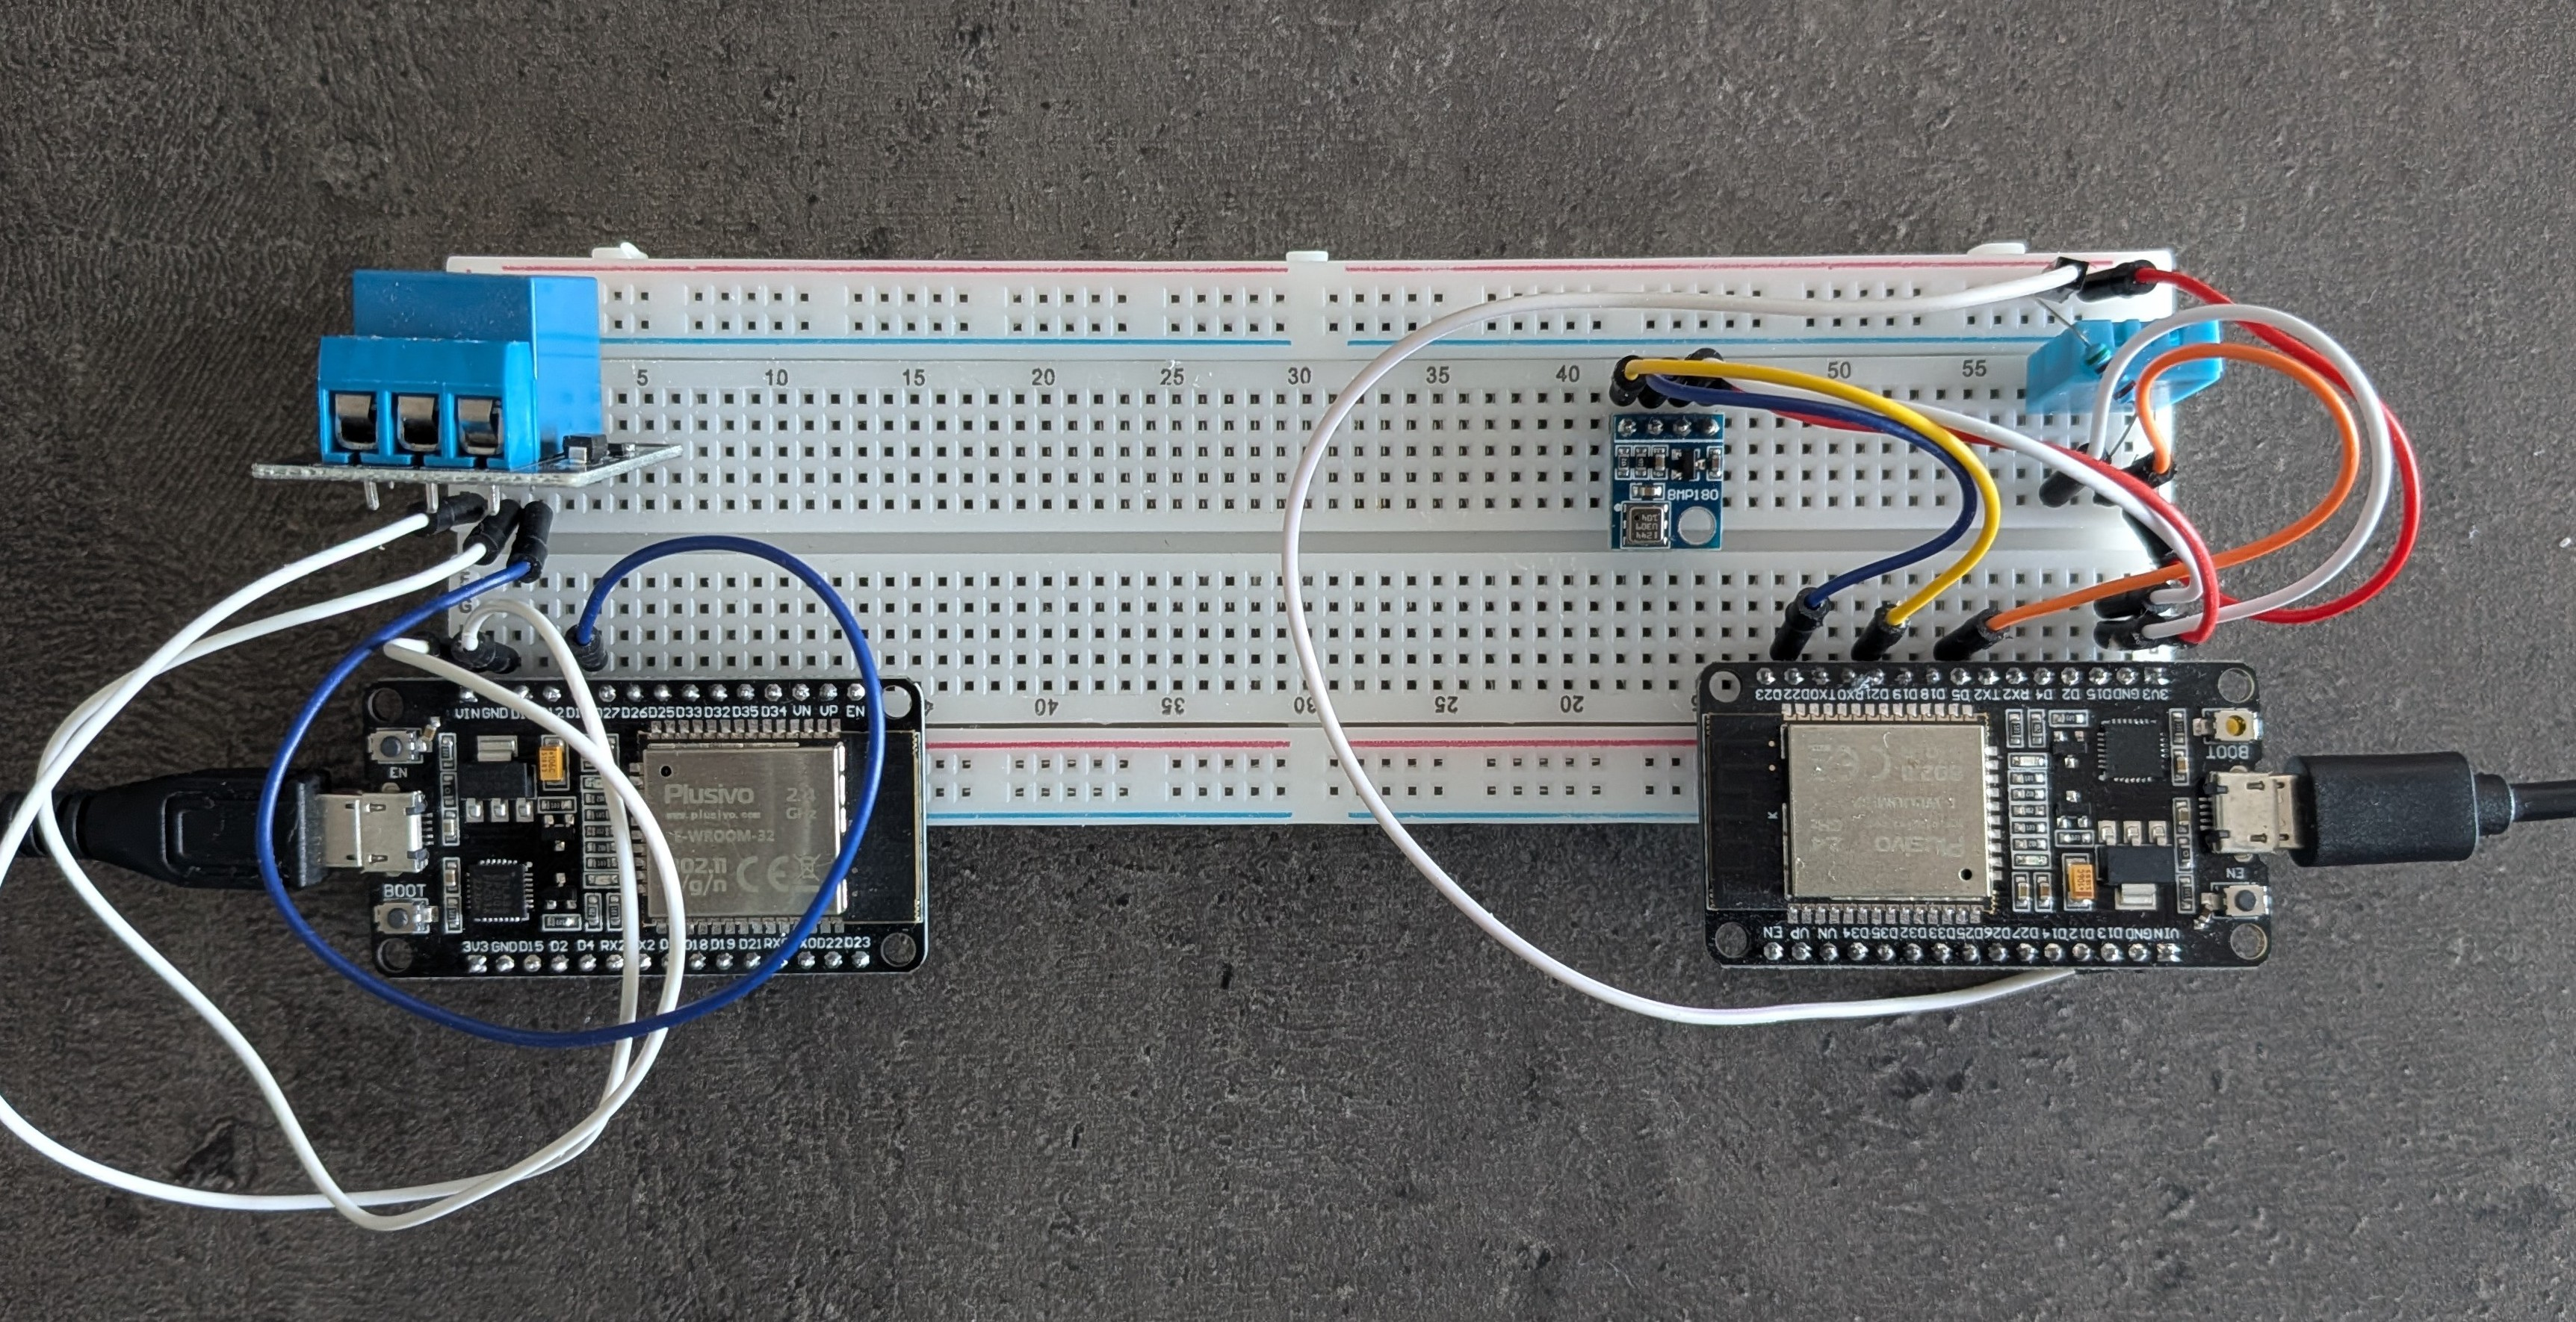
\includegraphics[width=0.7\textwidth]{figuri/esp32_devkit_overview.jpg}
    \caption{Modulul ESP32 DevKit V1 utilizat în prototipurile HomeForge}
    \label{fig:esp32_devkit}
\end{figure}

\section{Anatomia unui sketch HomeForge}
Toate variantele de firmware folosite de HomeForge sunt distribuite \emph{inline} în fișierul fixture \texttt{backend/api/fixtures/default\_device\_types.json}, sub câmpul \texttt{firmware\_code} al fiecărui tip de dispozitiv. Această structurare elimină dependența de un arbore de fișiere separat și permite ca distribuția unui set complet de tipuri (cod sursă, schemă electrică în Markdown și imagini codificate \texttt{base64}) să se reducă la o singură resursă JSON. Pentru a face explicațiile cât mai concrete, exemplele de mai jos provin din varianta \emph{ESP32 5V Relay}. Este singurul template care implementează ambele sensuri: fluxul de telemetrie (publicare de stare) și fluxul invers de comenzi (subscribe + callback). Astfel integrez ambele direcții de comunicație MQTT într-un singur fișier sursă. Pentru fluxurile pur senzoriale (publicare ciclică, fără recepție de comenzi), referințele vor merge către varianta \emph{ESP32 Thermostat DHT11 BMP180}.

\subsection{Variabile de configurare (placeholder-uri)}
Primele linii ale fiecărui sketch conțin trei constante marcate cu placeholder-uri Mustache-like:
\begin{minted}{cpp}
const char* wifi_ssid = "{{WIFI_SSID}}";
const char* wifi_password = "{{WIFI_PASSWORD}}";
const char* server_ip = "{{SERVER_IP}}";
const int mqtt_port = 1883;
\end{minted}
Aceste valori sunt înlocuite în clar de către utilizator înainte de compilare. \texttt{wifi\_ssid} și \texttt{wifi\_password} sunt strict obligatorii: backend-ul refuză să accepte un \texttt{firmware\_code} care nu conține referințele lor. În schimb, \texttt{server\_ip} a devenit \emph{opțional}: dispozitivul poate descoperi singur brokerul prin mDNS, mecanism descris în secțiunea \ref{sec:firmware-mdns}. Validatorul tratează valorile goale (\texttt{""} sau placeholder-ul ne-înlocuit) ca un semnal pentru activarea descoperirii automate, iar instalarea funcționează în acest caz fără ca utilizatorul să caute manual adresa serverului HomeForge.

\subsection{Identitatea dispozitivului: \texttt{deviceMac}}
La pornire, după conectarea la Wi-Fi, sketch-ul citește adresa MAC a interfeței Wi-Fi a cip-ului, o normalizează și se anunță în rețeaua locală prin mDNS:
\begin{minted}{cpp}
void setup_wifi() {
  delay(10);
  Serial.printf("\nConnecting to %s", wifi_ssid);
  WiFi.mode(WIFI_STA);
  WiFi.begin(wifi_ssid, wifi_password);
  while (WiFi.status() != WL_CONNECTED) {
    delay(500);
    Serial.print(".");
  }
  deviceIp  = WiFi.localIP().toString();
  deviceMac = WiFi.macAddress();
  deviceMac.replace(":", "");

  commandTopic = String("homeforge/devices/") + deviceMac + "/command";
  stateTopic   = String("homeforge/devices/") + deviceMac + "/state";

  String hostname = "homeforge-" + deviceMac;
  if (MDNS.begin(hostname.c_str())) {
    Serial.printf("mDNS responder started: %s.local\n", hostname.c_str());
  }
}
\end{minted}
La firmware-urile pur senzoriale, linia \texttt{commandTopic} lipsește (nu există nimic la care să se aboneze), restul fiind identic.
Patru detalii merită semnalate:
\begin{itemize}
    \item \texttt{WiFi.mode(WIFI\_STA)} forțează modul \emph{station-only}, oprind orice activitate de soft-AP rămasă din încercări anterioare;
    \item adresa MAC este formatată implicit de Arduino-ESP32 cu separatori (\texttt{:}); se elimină pentru ca topicul MQTT să fie un singur token alfanumeric, același format pe care îl așteaptă \texttt{mqtt\_listener} pe partea de Django;
    \item topicul \texttt{state} este construit pe toate firmware-urile; topicul \texttt{command} este construit doar de variantele care expun un actuator (\emph{ESP32 5V Relay}), restul fiind pur senzoriale și neavând nevoie să se aboneze la nimic;
    \item adresa MAC servește ca identificator unic la nivel de platformă: un dispozitiv care își schimbă IP-ul își păstrează identitatea către backend.
\end{itemize}

\subsection{Conectarea la broker și subscribe}
Funcția \texttt{reconnect()} este apelată din \texttt{loop()} ori de câte ori clientul \texttt{PubSubClient} pierde legătura. În varianta \emph{ESP32 5V Relay}, funcția înglobează și re-descoperirea brokerului atunci când adresa cache-uită nu mai răspunde:
\begin{minted}{cpp}
void reconnect() {
  while (!client.connected()) {
    if (strlen(mqttServer) == 0) {
      if (!discoverBroker()) { delay(3000); return; }
      client.setServer(mqttServer, mqtt_port);
    }
    Serial.printf("Connecting to MQTT broker %s ...", mqttServer);
    String clientId = "ESP32-Relay-" + deviceMac;
    if (client.connect(clientId.c_str())) {
      Serial.println(" connected!");
      client.subscribe(commandTopic.c_str());   // doar pe firmware-urile cu actuator
      publishState();
    } else {
      Serial.printf(" failed (rc=%d). Retrying in 5s...\n", client.state());
      delay(5000);
      return;
    }
  }
}
\end{minted}
\texttt{clientId} este unic per placă, construit din adresa MAC fără separatori și un prefix care identifică tipul de firmware: \texttt{ESP32-Relay-}, \texttt{ESP32-DHT11-}, \texttt{ESP32-BMP180-} sau \texttt{ESP32-Sensor-} (acesta din urmă pentru varianta combinată DHT11 + BMP180). Aceste prefixe sunt utile la depanare: un \texttt{mosquitto\_sub} pe brokerul HomeForge permite identificarea imediată a tipului de placă care s-a conectat. Imediat după conectare, dispozitivul publică starea curentă prin \texttt{publishState()}. Acest mesaj joacă rolul unui \emph{check-in}: este suficient pentru ca daemon-ul \texttt{mqtt\_listener} să facă auto-binding-ul descris în Capitolul 2. Firmware-urile pur senzoriale au aceeași structură, dar omit linia \texttt{client.subscribe(...)}: neavând actuator, nu se abonează la niciun topic de comandă.

\subsection{Telemetria: \texttt{publishState()}}
Funcția care construiește mesajul de stare folosește \texttt{ArduinoJson} pentru a serializa un document static. Pentru varianta \emph{ESP32 5V Relay}, mesajul publicat conține valoarea actuatorului (\texttt{relay\_1}), un eventual \emph{echo} către cheia dinamică folosită în comanda care a generat starea curentă și câmpurile auxiliare \texttt{ip} / \texttt{mac}:
\begin{minted}{cpp}
void publishState() {
  if (!client.connected()) return;

  StaticJsonDocument<256> doc;
  doc["ip"]  = deviceIp;
  doc["mac"] = deviceMac;
  doc[VAR_RELAY] = relayState;
  if (lastControlKey.length() > 0) {
    doc[lastControlKey] = relayState;   // trimite înapoi cheia dinamică
  }

  char buffer[256];
  serializeJson(doc, buffer);
  client.publish(stateTopic.c_str(), buffer);
}
\end{minted}
Mecanismul \emph{echo} acoperă cazul în care device builder-ul a generat o cheie dinamică pentru widget (de exemplu \texttt{switch-1780830762843}): firmware-ul reține ultima cheie primită în \texttt{lastControlKey} și o include în mesajul de stare alături de \texttt{relay\_1}, astfel încât interfața să vadă confirmarea pe identificatorul exact pe care l-a folosit la trimitere. Termostatele senzoriale (\emph{DHT11}, \emph{BMP180}, \emph{DHT11 + BMP180}) folosesc același tipar, dar populează câmpurile relevante pentru senzorii lor (\texttt{VAR\_TEMP}, \texttt{VAR\_HUMID}, \texttt{VAR\_PRESSURE}, după caz), fără \texttt{VAR\_RELAY} (nu au actuator). \texttt{StaticJsonDocument} cu dimensiune fixă alocă memoria în stivă, nu pe heap, ceea ce este recomandat pe microcontrolere unde fragmentarea heap-ului poate cauza eșecuri intermitente după ore de funcționare. Câmpurile \texttt{ip} și \texttt{mac} sunt incluse în payload chiar dacă brokerul le-ar putea infera din topic, fiind utile pentru auto-binding-ul descris în Capitolul 2, atunci când backend-ul nu cunoaște încă adresa MAC. Constantele de denumire a câmpurilor sunt declarate la începutul fiecărui sketch:
\begin{minted}{cpp}
const char* VAR_RELAY    = "relay_1";    // doar în ESP32 5V Relay
const char* VAR_TEMP     = "temperature";
const char* VAR_HUMID    = "humidity";
const char* VAR_PRESSURE = "pressure";
\end{minted}
Aceste nume sunt cele „standard", pe care \texttt{mqtt\_listener.map\_standard\_key()} le translatează către cheile dinamice ale widget-urilor.

\subsection{Recepția comenzilor: \texttt{callback()}}
Callback-ul \texttt{PubSubClient} este apelat de fiecare dată când brokerul publică un mesaj pe topicul la care firmware-ul s-a abonat. Implementarea concretă din \emph{ESP32 5V Relay} iterează peste cheile documentului JSON și acceptă, pe lângă \texttt{relay\_1}, orice identificator care începe cu prefixul \texttt{switch-} (folosit de device builder atunci când utilizatorul nu redenumește manual controlul). Parser-ul tolerează trei reprezentări pentru valoarea booleană (boolean nativ, string \texttt{"true"}, \texttt{"on"}, \texttt{"1"} și întreg), pentru a fi compatibil cu diferitele stiluri de payload pe care le poate genera UI-ul:
\begin{minted}{cpp}
void callback(char* topic, byte* payload, unsigned int length) {
  String message;
  for (unsigned int i = 0; i < length; i++) {
    message += (char)payload[i];
  }
  Serial.print("Command received: ");
  Serial.println(message);

  StaticJsonDocument<256> doc;
  if (deserializeJson(doc, message)) return;

  JsonObject root = doc.as<JsonObject>();
  for (JsonPair kv : root) {
    String key = kv.key().c_str();
    if (key == VAR_RELAY || key.startsWith("switch-")) {
      lastControlKey = key;
      if (kv.value().is<bool>()) {
        relayState = kv.value().as<bool>();
      } else if (kv.value().is<const char*>()) {
        String val = kv.value().as<String>();
        val.toLowerCase();
        relayState = (val == "true" || val == "on" || val == "1");
      } else if (kv.value().is<int>()) {
        relayState = kv.value().as<int>() == 1;
      }
      break;
    }
  }

  digitalWrite(RELAY_PIN, relayState ? HIGH : LOW);

  preferences.begin("state", false);
  preferences.putBool("relay", relayState);
  preferences.end();

  publishState();
}
\end{minted}
Trei detalii merită observate. Primul: variabila \texttt{lastControlKey} reține identificatorul exact cu care a venit ultima comandă, pentru ca \texttt{publishState()} să poată face \emph{echo} înapoi pe aceeași cheie dinamică (mecanism prezentat în subsecțiunea anterioară). Al doilea: după acționarea releului, starea este persistată în memoria nevolatilă a ESP32 (\texttt{Preferences}, namespace \texttt{state}), astfel încât după o reală cădere de tensiune dispozitivul revine în aceeași stare la pornire. Al treilea: \texttt{publishState()} este apelat imediat după execuție, închizând bucla de feedback: backend-ul primește confirmarea că operația a fost realizată și actualizează \texttt{current\_state} în baza de date, iar frontend-ul preia noua valoare la următoarea iterație de \texttt{refetchInterval} (3 secunde).

\subsection{Bucla principală}
\texttt{loop()} este structurată în trei pași: servirea serverului HTTP de fallback (\texttt{server.handleClient()} pentru endpoint-ul \texttt{/config}), asigurarea conexiunii MQTT prin \texttt{reconnect()} și o secvență ciclică de eșantionare la fiecare câteva secunde. Pentru \emph{ESP32 5V Relay}, partea ciclică se limitează la republicarea stării actuatorului (nu există senzori de citit); pentru firmware-urile de termostat, citirea senzorilor este izolată într-o funcție \texttt{readSensors()} apelată din bucla principală. Schema buclei pentru varianta \emph{ESP32 Thermostat DHT11 BMP180}:
\begin{minted}{cpp}
void loop() {
  server.handleClient();
  if (!client.connected()) {
    reconnect();
  }
  client.loop();

  unsigned long now = millis();
  if (now - lastMsg > interval) {
    lastMsg = now;
    readSensors();
    publishState();
  }
}

void readSensors() {
  float newT = dht.readTemperature();
  float newH = dht.readHumidity();
  float newP = bmp.readPressure();

  if (!isnan(newT) && !isnan(newH)) {
    humidity = newH;
    // Aplică corecția de toleranță DHT11.
    temperature = (DHT11_ERROR < 0) ? newT + DHT11_ERROR : newT - DHT11_ERROR;
    if (!isnan(newP)) pressure = newP / 100.0;   // Pa în hPa
  } else {
    Serial.println("Failed to read from DHT11/BMP180 sensor!");
  }
}
\end{minted}
Constanta \texttt{interval = 5000} (5 secunde) este sincronizată cu pragul din \texttt{mqtt\_listener.check\_offline\_devices()} (30 de secunde): primim 6 oportunități de heartbeat ratate înainte ca dispozitivul să fie declarat offline. Pe DHT11, citirile prea frecvente nu sunt fiabile (senzorul are nevoie de cel puțin o secundă între eșantioane), deci intervalul de 5 secunde oferă o marjă confortabilă. Verificarea \texttt{!isnan(newT) \&\& !isnan(newH)} reține valorile vechi atunci când o citire eșuează intermitent, iar constanta \texttt{DHT11\_ERROR} aplică o corecție de offset pentru a compensa eroarea sistematică observată la lotul de DHT11 folosit. Presiunea barometrică este convertită din Pascali (unitate brută a BMP180) în hectopascali (\texttt{hPa}), unitatea uzuală în meteorologie.

\section{Descoperirea automată a brokerului prin mDNS}
\label{sec:firmware-mdns}
Una dintre operațiunile mai puțin elegante în implementarea inițială era cerința ca utilizatorul să cunoască adresa IP a serverului HomeForge înainte de compilare. Pentru rețelele în care IP-ul serverului este atribuit dinamic prin DHCP, această cerință devenea o sursă recurentă de probleme: o singură reasignare DHCP forța re-flash-area tuturor dispozitivelor. Versiunea curentă rezolvă acest aspect prin introducerea unui mecanism de descoperire automată bazat pe Multicast DNS (mDNS) și DNS-Based Service Discovery (DNS-SD), conform RFC 6762 \cite{rfc_mdns} și RFC 6763 \cite{rfc_dnssd}.

\subsection{Principiul de funcționare}
mDNS permite rezolvarea numelor DNS pe segmentul local de rețea fără a depinde de un server DNS centralizat, prin trimiterea de pachete UDP către adresa de multicast \texttt{224.0.0.251} (IPv4), pe portul 5353. DNS-SD extinde acest mecanism cu o convenție pentru descoperirea serviciilor: un client interesat de un serviciu de tipul „MQTT peste TCP" interoghează numele rezervat \texttt{\_mqtt.\_tcp.local}, iar furnizorii de serviciu răspund cu o înregistrare SRV care indică gazda și portul efectiv. HomeForge folosește această convenție prin daemon-ul Avahi care rulează în containerul backend (acolo unde topologia de rețea o permite, vezi Capitolul 5), publicând în mod continuu un record \texttt{\_mqtt.\_tcp} cu portul 1883.

\subsection{Ierarhia celor trei niveluri de descoperire}
Firmware-ul ESP32 încearcă să identifice brokerul printr-o secvență de trei mecanisme, în ordinea priorității:

\begin{enumerate}
    \item \textbf{Override manual prin \texttt{server\_ip}.} Dacă utilizatorul a substituit explicit adresa serverului la momentul compilării, dispozitivul se conectează direct, fără descoperire. Modul este util pentru topologii fixe sau pentru sisteme unde mDNS nu este disponibil.
    \item \textbf{Cache local în memorie nevolatilă (NVS).} La fiecare conectare reușită, firmware-ul salvează adresa brokerului în NVS folosind biblioteca \texttt{Preferences}. La un \texttt{reboot} ulterior, reconectarea este aproape instantanee fiindcă cache-ul este consultat înainte de a iniția o nouă interogare multicast.
    \item \textbf{Interogare mDNS / DNS-SD.} Atunci când \texttt{server\_ip} este gol și cache-ul lipsește sau este invalid, firmware-ul folosește biblioteca \texttt{ESPmDNS} pentru a interoga \texttt{\_mqtt.\_tcp} pe segmentul de rețea. Funcția \texttt{discoverBroker()} încearcă până la trei interogări consecutive (cu timeout scurt) și acceptă primul răspuns valid:
\end{enumerate}

\begin{minted}{cpp}
bool discoverBroker() {
  Serial.println("Discovering HomeForge broker via mDNS...");
  for (int attempt = 0; attempt < 3; attempt++) {
    int n = MDNS.queryService(MDNS_SERVICE, MDNS_PROTO);
    if (n > 0) {
      IPAddress ip = MDNS.address(0);
      String found = ip.toString();
      if (found != "0.0.0.0") {
        strncpy(mqttServer, found.c_str(), sizeof(mqttServer) - 1);
        saveBroker(found);
        Serial.printf("Broker found: %s\n", mqttServer);
        return true;
      }
    }
    delay(1000);
  }
  Serial.println("Broker not found (will retry / use /config fallback).");
  return false;
}
\end{minted}
\texttt{mqttServer} este un buffer de caractere global (umplut prin \texttt{strncpy}), iar \texttt{saveBroker(found)} apelează API-ul \texttt{Preferences} pentru a persista adresa descoperită în memoria nevolatilă a ESP32, pentru reutilizare la următorul boot.

Dacă toate cele trei niveluri eșuează (situație rară, dar plauzibilă atunci când serverul nu rulează încă sau este pe altă subrețea), dispozitivul activează un al patrulea mecanism de rezervă: pornește un server HTTP pe portul 80 și acceptă o cerere \texttt{POST /config} cu adresa brokerului. Utilizatorul deschide în browser pagina dispozitivului și introduce adresa manual, fără a fi necesar un reflash.

\subsection{Anunțarea propriei identități prin mDNS}
Pe lângă consumarea înregistrărilor mDNS, fiecare dispozitiv își publică și propria identitate, sub un nume derivat din adresa MAC: \texttt{esp32-<MAC>.local}. Astfel, administratorul rețelei locale poate accesa dispozitivul prin nume DNS, fără a căuta IP-ul în interfața de administrare a router-ului. Apelul \texttt{MDNS.begin(hostname)} se face imediat după conectarea la Wi-Fi, în secvența standard de inițializare.
Setul predefinit conține patru tipuri de dispozitive ESP32, toate stocate inline în \texttt{backend/api/fixtures/default\_device\_types.json} și importate automat la apelul \texttt{POST /api/device-types/import-defaults/} în prima sesiune cu administratorul. Fiecare intrare conține integral codul firmware Arduino, schema electrică (text Markdown + imagine \texttt{base64}), documentația și definiția vizuală a cardului, totul într-un singur obiect JSON, fără referințe către fișiere externe.

Cele patru variante împart o singură categorie funcțională clară. \textbf{ESP32 5V Relay} este singurul template care expune un actuator: un releu controlat de \texttt{RELAY\_PIN = GPIO 14}, redat în interfață printr-un widget \texttt{TOGGLE} a cărui variabilă (\texttt{relay\_1} sau un identificator generat dinamic care începe cu prefixul \texttt{switch-}) este transmisă bidirecțional, atât în publicările de stare cât și în comenzile primite de la backend. Celelalte trei variante sunt strict senzoriale: publică telemetrie ciclică, fără a se abona la topicul de comandă și fără a implementa un \texttt{callback} de recepție.

\textbf{ESP32 Thermostat DHT11} folosește un senzor DHT11 (temperatură + umiditate) conectat la \texttt{DHTPIN = GPIO 5} și expune două widget-uri: \texttt{TEMPERATURE} și \texttt{HUMIDITY}. \textbf{ESP32 Temperature \& Pressure BMP180} folosește un senzor BMP180 pe magistrală I2C (\texttt{SDA = GPIO 21}, \texttt{SCL = GPIO 22}, valorile implicite Wire ale ESP32), publicând temperatura măsurată de BMP-ul însuși și presiunea barometrică în două widget-uri \texttt{TEMPERATURE} și \texttt{PRESSURE}. \textbf{ESP32 Thermostat DHT11 BMP180} combină cele două: DHT11 pe GPIO 5 și BMP180 pe magistrala I2C standard, publicând trei valori (temperatură, umiditate și presiune) în trei widget-uri corespunzătoare.

Cheile cu care fiecare firmware publică datele pe broker sunt constantele \texttt{VAR\_TEMP = "temperature"}, \texttt{VAR\_HUMID = "humidity"}, \texttt{VAR\_PRESSURE = "pressure"} și \texttt{VAR\_RELAY = "relay\_1"}. Daemon-ul \texttt{mqtt\_listener} de pe partea de backend mapează aceste nume canonice către identificatorii dinamici generați de device builder pentru fiecare widget al cardului, astfel încât reorganizarea widget-urilor în UI nu impune reflash-area firmware-ului.

Pentru fiecare variantă, schema electrică este distribuită ca imagine \texttt{base64} în câmpul \texttt{wiring\_diagram\_base64} al obiectului JSON, însoțită opțional de o descriere textuală în \texttt{wiring\_diagram\_text}. Schema electrică minimală pentru varianta \emph{ESP32 5V Relay} este sintetizată în Tabelul \ref{tab:esp32_relay_pinout}, iar montajele pe breadboard ale tuturor celor patru variante sunt arătate în Figura \ref{fig:wiring_diagrams}:
\begin{table}[htb]
    \centering
        \renewcommand{\arraystretch}{1.2}
    \small
    \begin{tabular}{|l|l|l|l|}
        \hline
        \textbf{Modul} & \textbf{Pin} & \textbf{ESP32} & \textbf{Descriere} \\ \hline
        Releu & VCC & 5V & Alimentare 5 V \\ \hline
        Releu & GND & GND & Masă \\ \hline
        Releu & IN  & GPIO 14 & Semnal de control (\texttt{RELAY\_PIN}) \\ \hline
    \end{tabular}
    \caption{Conexiunile pinilor pentru tipul \emph{ESP32 5V Relay}}
    \label{tab:esp32_relay_pinout}
\end{table}

\begin{figure}[htb]
    \centering
    \begin{subfigure}[t]{0.48\textwidth}
        \centering
        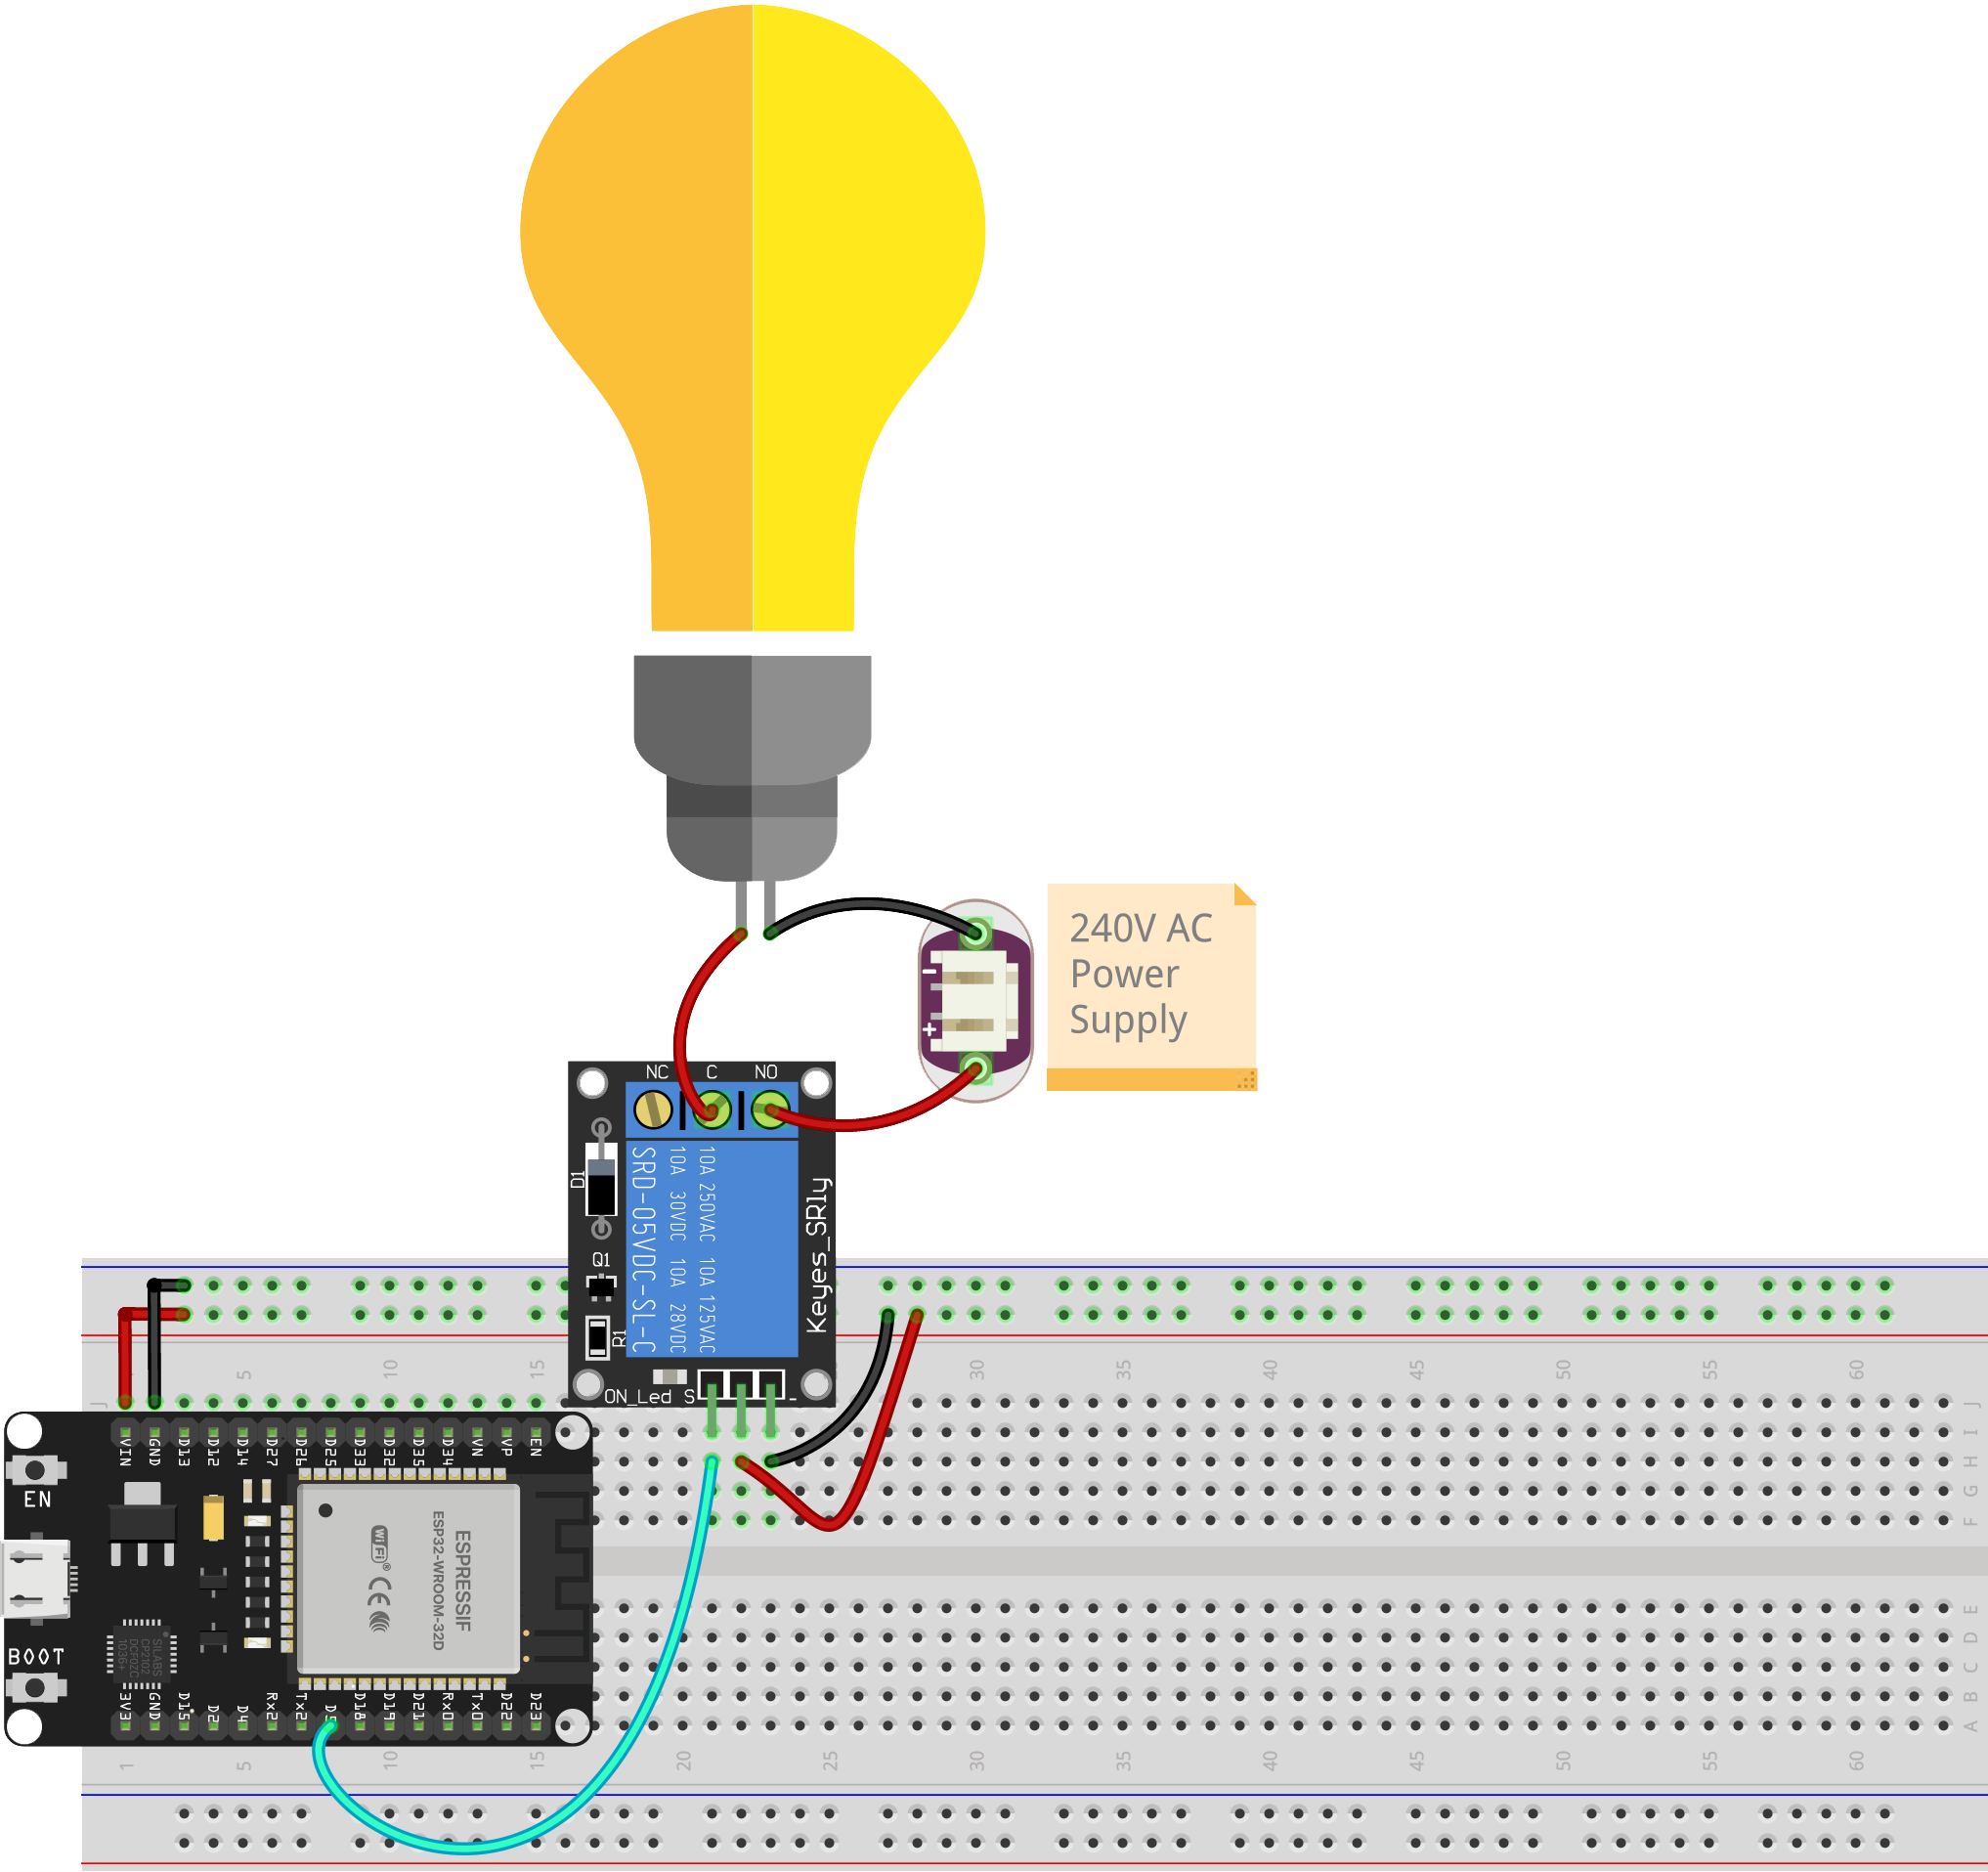
\includegraphics[width=\linewidth]{figuri/breadboard_esp32_relay.png}
        \caption{ESP32 5V Relay}
        \label{fig:wiring_relay}
    \end{subfigure}\hfill
    \begin{subfigure}[t]{0.48\textwidth}
        \centering
        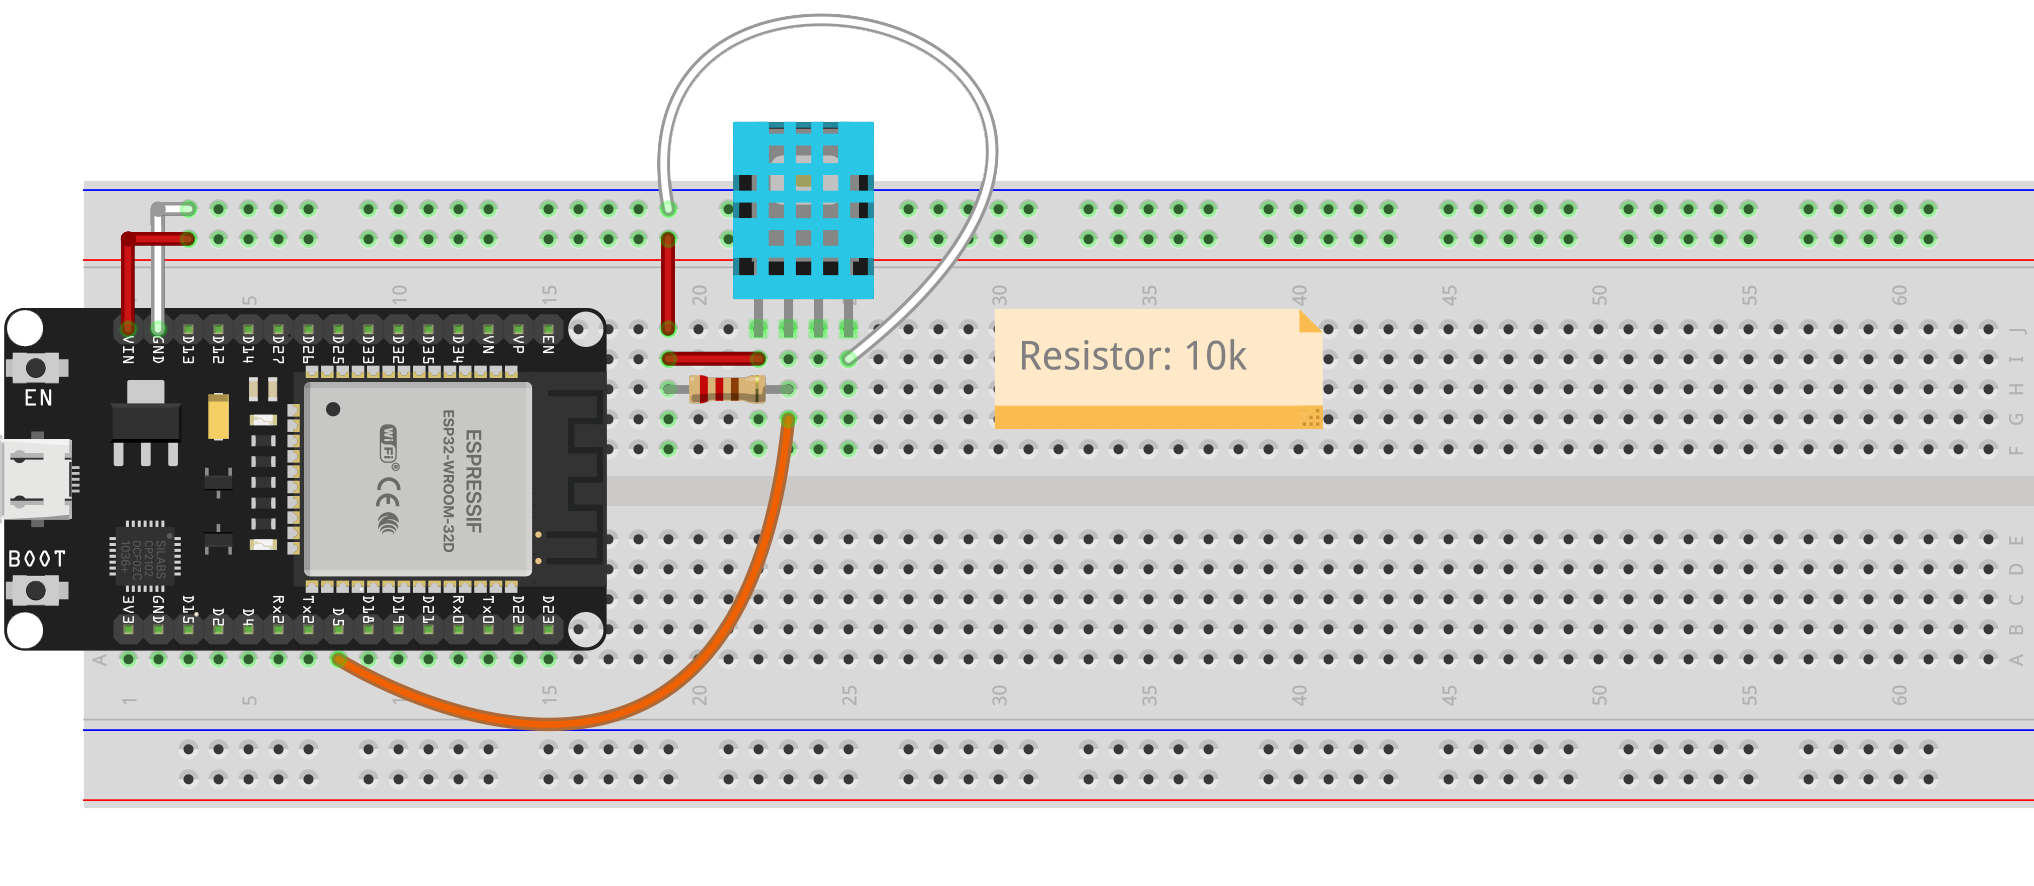
\includegraphics[width=\linewidth]{figuri/breadboard_esp32_thermostat_dht11.png}
        \caption{ESP32 Thermostat DHT11}
        \label{fig:wiring_dht11}
    \end{subfigure}

    \vspace{0.6em}

    \begin{subfigure}[t]{0.48\textwidth}
        \centering
        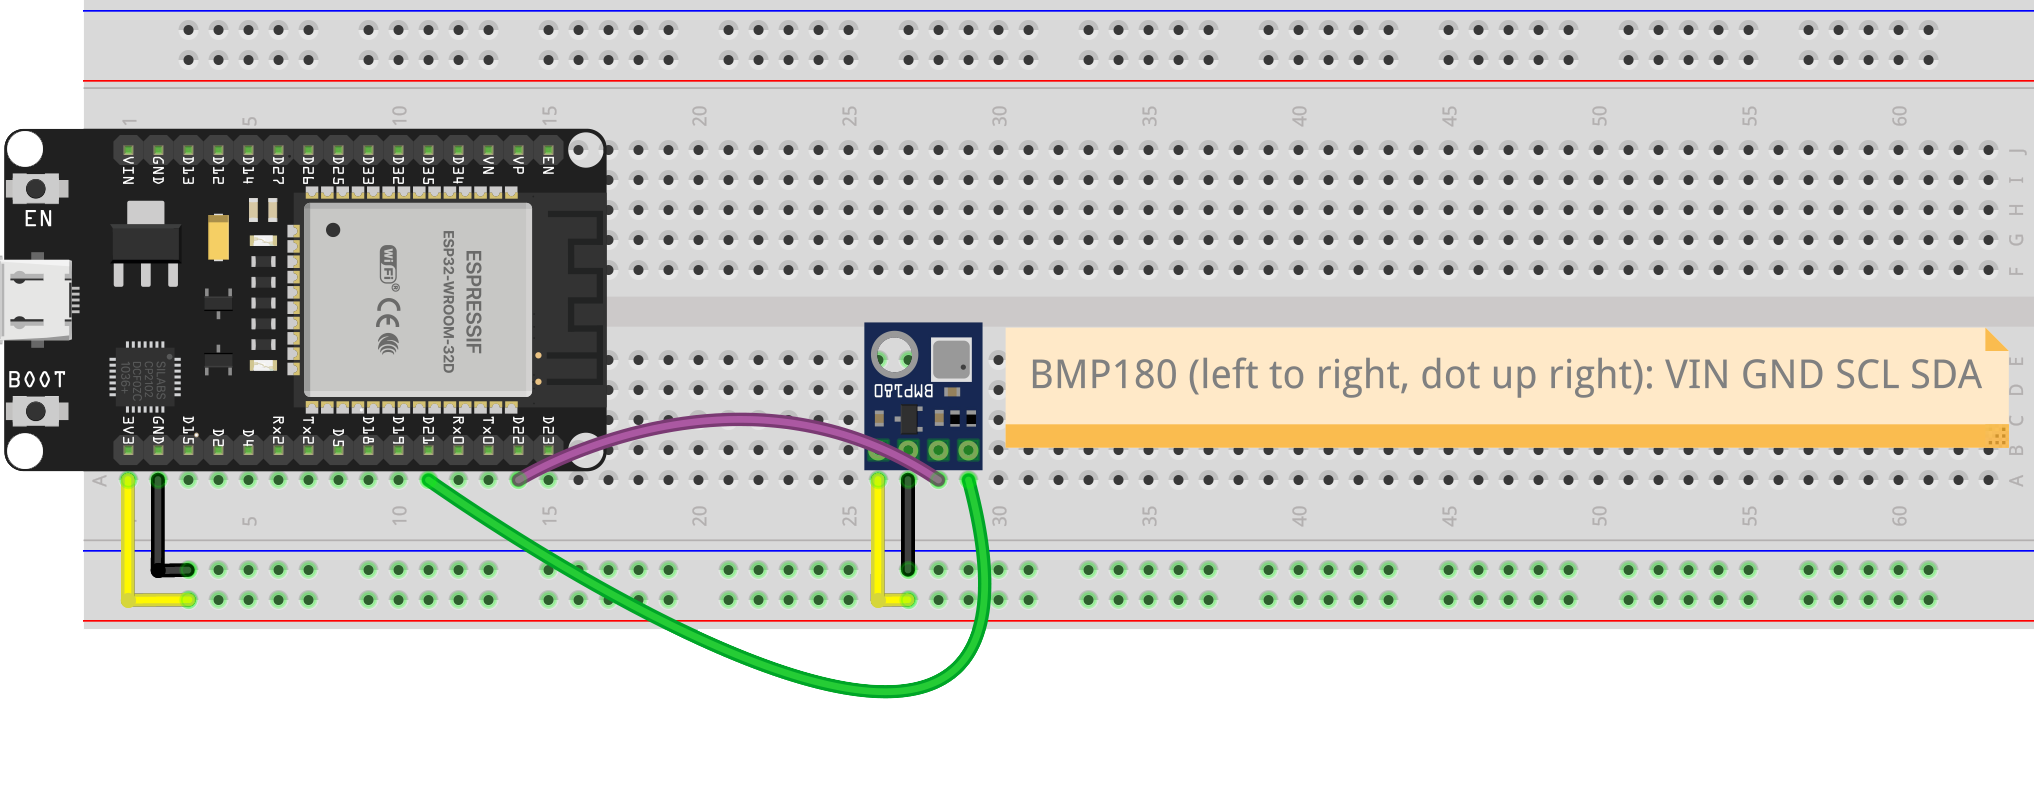
\includegraphics[width=\linewidth]{figuri/breadboard_esp32_thermostat_bmp180.png}
        \caption{ESP32 Temperature \& Pressure BMP180}
        \label{fig:wiring_bmp180}
    \end{subfigure}\hfill
    \begin{subfigure}[t]{0.48\textwidth}
        \centering
        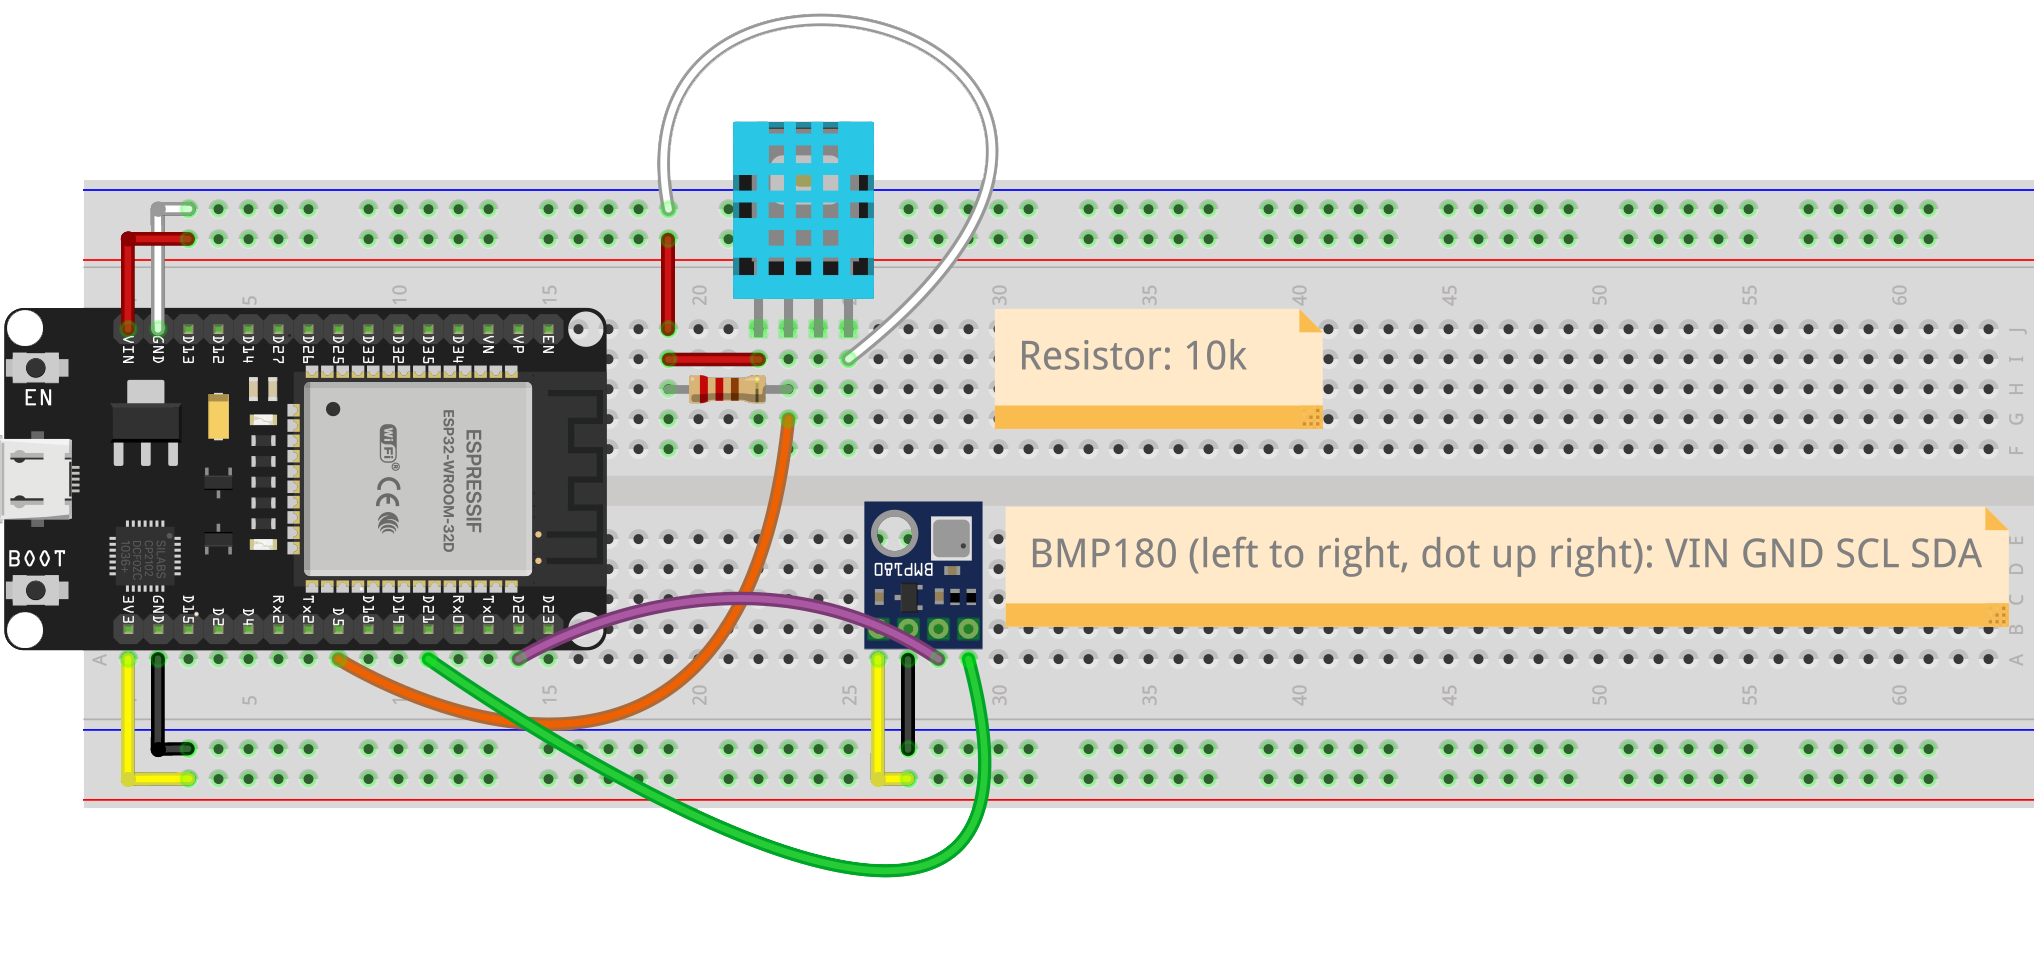
\includegraphics[width=\linewidth]{figuri/breadboard_esp32_thermostat_dht11_bmp180.png}
        \caption{ESP32 Thermostat DHT11 + BMP180}
        \label{fig:wiring_dht11_bmp180}
    \end{subfigure}
    \caption{Schemele de conexiuni (breadboard) ale celor patru tipuri de dispozitive predefinite: releul 5V comandând un consumator (a), termostatul cu DHT11 (b), modulul de temperatură și presiune BMP180 pe I2C (c) și varianta combinată DHT11 + BMP180 (d).}
    \label{fig:wiring_diagrams}
\end{figure}

\FloatBarrier
\section{Bibliotecile Arduino utilizate}
Pentru a compila firmware-urile, mediul Arduino IDE folosește mai multe biblioteci. O parte sunt incluse automat cu pachetul ESP32 Arduino Core de la Espressif: \texttt{WiFi.h} pentru conectarea Wi-Fi, \texttt{ESPmDNS.h} pentru descoperirea automată a brokerului, \texttt{Preferences.h} pentru cache-ul persistent al adresei brokerului în memoria nevolatilă, \texttt{WebServer.h} pentru endpoint-ul de fallback \texttt{/config} și \texttt{Wire.h} pentru comunicarea I2C. Restul se instalează prin \emph{Library Manager}: \texttt{PubSubClient} (Nick O'Leary, client MQTT cu suport pentru QoS 0 și 1), \texttt{ArduinoJson} (Benoit Blanchon, parsing și serializare JSON cu documente alocate static), \texttt{DHT sensor library} (Adafruit, folosită în firmware-urile cu DHT11) și \texttt{Adafruit BMP085 Library} (Adafruit, compatibilă cu BMP180). Pachetul ESP32 Arduino Core se adaugă în Arduino IDE prin \emph{File → Preferences → Additional Boards Manager URLs}, cu URL-ul oficial \texttt{https://espressif.github.io/arduino-esp32/package\_esp32\_index.json}.

\section{Limitări ale implementării curente}
Pentru claritate, enumăr aici ce nu este implementat în firmware-ul curent. Nu folosesc task-uri FreeRTOS create explicit: bucla \texttt{loop()} împreună cu \texttt{PubSubClient.loop()} acoperă volumul actual de logică. Nu există un \texttt{Captive Portal} pentru configurarea Wi-Fi la prima pornire, SSID-ul și parola fiind înlocuite direct în cod prin placeholder-uri. Comunicarea MQTT nu folosește TLS, ceea ce este acceptabil într-un LAN privat, dar pentru un deployment de producție ar trebui adăugate certificate și \texttt{WiFiClientSecure}. Actualizarea OTA nu este implementată, re-flash-area făcându-se prin USB-UART. Niciuna dintre aceste limitări nu împiedică utilizarea curentă a platformei și sunt menționate ca direcții posibile de extindere.